

\documentclass[12pt]{article}
\usepackage{amsmath}
\usepackage{latexsym}
\usepackage{amsfonts}
\usepackage[normalem]{ulem}
\usepackage{array}
\usepackage{amssymb}
\usepackage{graphicx}
\usepackage[backend=biber,
style=numeric,
sorting=none,
isbn=false,
doi=false,
url=false,
]{biblatex}\addbibresource{bibliography.bib}

\usepackage{subfig}
\usepackage{wrapfig}
\usepackage{wasysym}
\usepackage{enumitem}
\usepackage{adjustbox}
\usepackage{ragged2e}
\usepackage[svgnames,table]{xcolor}
\usepackage{tikz}
\usepackage{longtable}
\usepackage{changepage}
\usepackage{setspace}
\usepackage{hhline}
\usepackage{multicol}
\usepackage{tabto}
\usepackage{float}
\usepackage{multirow}
\usepackage{makecell}
\usepackage{fancyhdr}
\usepackage[toc,page]{appendix}
\usepackage[hidelinks]{hyperref}
\usetikzlibrary{shapes.symbols,shapes.geometric,shadows,arrows.meta}
\tikzset{>={Latex[width=1.5mm,length=2mm]}}
\usepackage{flowchart}\usepackage[paperheight=11.0in,paperwidth=8.5in,left=0.79in,right=0.79in,top=0.79in,bottom=0.79in,headheight=1in]{geometry}
\usepackage[utf8]{inputenc}
\usepackage[T1]{fontenc}
\TabPositions{0.49in,0.98in,1.47in,1.96in,2.45in,2.94in,3.43in,3.92in,4.41in,4.9in,5.39in,5.88in,6.37in,6.86in,}

\urlstyle{same}


 


\setcounter{tocdepth}{5}
\setcounter{secnumdepth}{5}





\setlistdepth{9}
\renewlist{enumerate}{enumerate}{9}
		\setlist[enumerate,1]{label=\arabic*)}
		\setlist[enumerate,2]{label=\alph*)}
		\setlist[enumerate,3]{label=(\roman*)}
		\setlist[enumerate,4]{label=(\arabic*)}
		\setlist[enumerate,5]{label=(\Alph*)}
		\setlist[enumerate,6]{label=(\Roman*)}
		\setlist[enumerate,7]{label=\arabic*}
		\setlist[enumerate,8]{label=\alph*}
		\setlist[enumerate,9]{label=\roman*}

\renewlist{itemize}{itemize}{9}
		\setlist[itemize]{label=$\cdot$}
		\setlist[itemize,1]{label=\textbullet}
		\setlist[itemize,2]{label=$\circ$}
		\setlist[itemize,3]{label=$\ast$}
		\setlist[itemize,4]{label=$\dagger$}
		\setlist[itemize,5]{label=$\triangleright$}
		\setlist[itemize,6]{label=$\bigstar$}
		\setlist[itemize,7]{label=$\blacklozenge$}
		\setlist[itemize,8]{label=$\prime$}

\setlength{\topsep}{0pt}\setlength{\parindent}{0pt}
\renewcommand{\arraystretch}{1.3}


%%%%%%%%%%%%%%%%%%%% Document code starts here %%%%%%%%%%%%%%%%%%%%



\begin{document}

\vspace{\baselineskip}

\vspace{\baselineskip}
\begin{adjustwidth}{0.0in}{0.01in}
{\fontsize{16pt}{19.2pt}\selectfont Universidad Politécnica de la Zona Metropolitana de Guadalajara\par}\par

\end{adjustwidth}

\begin{adjustwidth}{0.0in}{0.01in}
{\fontsize{16pt}{19.2pt}\selectfont Jesús David Esparza Cabrera\par}\par

\end{adjustwidth}


\vspace{\baselineskip}
\begin{adjustwidth}{0.0in}{0.01in}
{\fontsize{16pt}{19.2pt}\selectfont 5 de Noviembre del 2019\par}\par

\end{adjustwidth}


\vspace{\baselineskip}
\begin{adjustwidth}{0.0in}{0.01in}
{\fontsize{16pt}{19.2pt}\selectfont \textcolor[HTML]{21409A}{Diseño y fabricación de 3 PCB con Optoacopladores, Transistores, Relevadores como dispositivo de interfaz y probarla en la práctica 10}\par}\par

\end{adjustwidth}



%%%%%%%%%%%%%%%%%%%% Figure/Image No: 1 starts here %%%%%%%%%%%%%%%%%%%%

\begin{figure}[H]
	\begin{Center}
		
\includegraphics[width=5.06in,height=5.51in]{./media/image1.png}
	\end{Center}
\end{figure}


%%%%%%%%%%%%%%%%%%%% Figure/Image No: 1 Ends here %%%%%%%%%%%%%%%%%%%%

\par


\vspace{\baselineskip}

\vspace{\baselineskip}

\vspace{\baselineskip}

\vspace{\baselineskip}

\vspace{\baselineskip}

\vspace{\baselineskip}

\vspace{\baselineskip}

\vspace{\baselineskip}

\vspace{\baselineskip}

\vspace{\baselineskip}

\vspace{\baselineskip}

\vspace{\baselineskip}

\vspace{\baselineskip}

\vspace{\baselineskip}

\vspace{\baselineskip}

\vspace{\baselineskip}

\vspace{\baselineskip}

\vspace{\baselineskip}

\vspace{\baselineskip}

\vspace{\baselineskip}
\begin{adjustwidth}{0.0in}{0.01in}
{\fontsize{17pt}{20.4pt}\selectfont \textcolor[HTML]{21409A}{Fabricación de Circuitos Impresos (PCB)}\par}\par

\end{adjustwidth}

\begin{adjustwidth}{0.0in}{0.01in}
Al diseñar un proyecto o prototipo electrónico, primero se debe probar, armándose en una placa de pruebas o protoboard. Cuando funcione correctamente, se  dibujará el diagrama esquemático, ya sea a mano, o en computador, usando programas especializados como el proteus, eagle o Pspice.  Posteriormente se diseña y fabrica el circuito impreso (PCB), y para finalizar, se montan los componentes en la tarjeta, para finalmente colocarlo en un chasis o gabinete, que le darán una presentación final a nuestro proyecto.\par

\end{adjustwidth}

Prueba del circuito en la placa de pruebas o protoboard\par



%%%%%%%%%%%%%%%%%%%% Figure/Image No: 2 starts here %%%%%%%%%%%%%%%%%%%%

\begin{figure}[H]
	\begin{Center}
		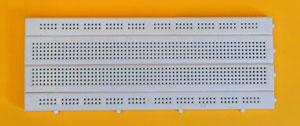
\includegraphics[width=3.15in,height=1.33in]{./media/image2.jpeg}
	\end{Center}
\end{figure}


%%%%%%%%%%%%%%%%%%%% Figure/Image No: 2 Ends here %%%%%%%%%%%%%%%%%%%%

\par

La placa de pruebas (en ingles protoboard), es una herramienta de estudio en la  electrónica, que permite interconectar los componentes electrónicos; ya sean resistencias, condensadores, semiconductores, etc, sin necesidad de soldarlos en un impreso, permitiendo así, hacer infinidad de pruebas de manera fácil, alcanzando la optimización deseada del circuito.\par



%%%%%%%%%%%%%%%%%%%% Figure/Image No: 3 starts here %%%%%%%%%%%%%%%%%%%%

\begin{figure}[H]
	\begin{Center}
		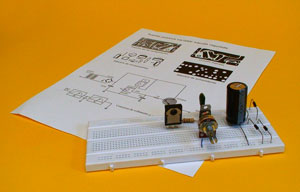
\includegraphics[width=3.15in,height=2.02in]{./media/image3.jpeg}
	\end{Center}
\end{figure}


%%%%%%%%%%%%%%%%%%%% Figure/Image No: 3 Ends here %%%%%%%%%%%%%%%%%%%%

\par

La placa de prueba está compuesta por segmentos plásticos con perforaciones y láminas delgadas de una aleación de cobre, estaño y fósforo, las cuales pasan por debajo de las perforaciones, creando una serie de líneas de conducción paralelas. Estas líneas están distribuidas; unas en forma transversal y otras longitudinalmente. Las líneas transversales están interrumpidas en la parte central de la placa, para facilitar la inserción de circuitos integrados tipo DIP (Dual Inline Packages), y que cada pata del circuito integrado, tenga una línea de conexión por separado. En la cara opuesta de la placa, trae un forro con pegante, que sirve para sellar y mantener en su lugar las láminas metálicas.\\
Al momento de hacer un circuito en el protoboard, se utilizan las láminas transversales para interconectar los componentes y las longitudinales para su alimentación.\par

El diagrama esquemático (schematic)\par



%%%%%%%%%%%%%%%%%%%% Figure/Image No: 4 starts here %%%%%%%%%%%%%%%%%%%%

\begin{figure}[H]
	\begin{Center}
		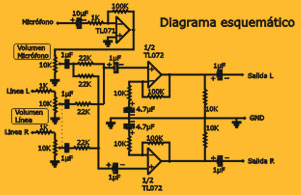
\includegraphics[width=3.14in,height=2.03in]{./media/image4.jpeg}
	\end{Center}
\end{figure}


%%%%%%%%%%%%%%%%%%%% Figure/Image No: 4 Ends here %%%%%%%%%%%%%%%%%%%%

\par

Cuando el circuito está funcionando a la perfección en el protoboard, se procede ha realizar el diagrama esquemático. Esto consiste en dibujar el circuito, utilizando los símbolos electrónicos. Se puede hacer a mano, o en el computador, utilizando programas como el proteus, workbench, Pspice, Eagle, etc. Los diagramas e impresos realizados para nuestro sitio Web, son dibujados en Corel draw, programa de creación de gráficos vectoriales, el cual da una excelente resolución a la hora de imprimir.\\
Nota: Es necesario tener un buen conocimiento de simbología electrónica, para hacer el diagrama esquemático sin errores.\par

Diseño y fabricación de circuitos impresos\par



%%%%%%%%%%%%%%%%%%%% Figure/Image No: 5 starts here %%%%%%%%%%%%%%%%%%%%

\begin{figure}[H]
	\begin{Center}
		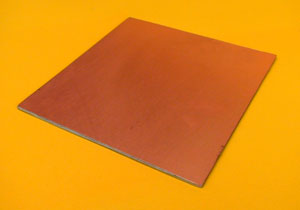
\includegraphics[width=3.15in,height=2.21in]{./media/image5.jpeg}
	\end{Center}
\end{figure}


%%%%%%%%%%%%%%%%%%%% Figure/Image No: 5 Ends here %%%%%%%%%%%%%%%%%%%%

\par

Comencemos por hablar un poco del material de los circuitos impresos. Uno de los materiales más usado para la fabricación de circuitos impresos o también llamada placa fenólica, es la baquelita (en ingles Bakelite), un feno-plástico resistente al calor y a los solventes, desarrollado por el belga-americano, Leo Hendrik Baekeland, entre 1902 y 1907. También se usa la fibra de vidriocon resina de poliéster, en la fabricación de circuitos impresos. Esta es más costosa, pero de mejor calidad y presentación.\\
Cualquiera de estos dos materiales, llevan un baño de cobre en una o en ambas caras. La función del cobre es conducir la electricidad. Al momento de hacer un circuito impreso, la tarjeta; ya sea en baquelita o en fibra de vidrio, el cobre de esta, tendrá la forma de $``$caminos$"$ , los cuales interconectarán los componentes que irán en la tarjeta.\par

Técnicas para la fabricación de los circuitos impresos\par

Existen diferentes técnicas para la fabricación de los circuitos impresos (PCB). Dependiendo de nuestro presupuesto y objetivo, escogemos la técnica que más nos convenga. Las técnicas más conocidas son:\par

– Elaboración de circuitos impresos con tinta indeleble\\
– Elaboración de circuitos impresos con la técnica de planchado (papel termo transferible, impresión láser)\\
– Elaboración de circuitos impresos con la técnica de serigrafía.\par

Elaboración de circuitos impresos con tinta indeleble\par



%%%%%%%%%%%%%%%%%%%% Figure/Image No: 6 starts here %%%%%%%%%%%%%%%%%%%%

\begin{figure}[H]
	\begin{Center}
		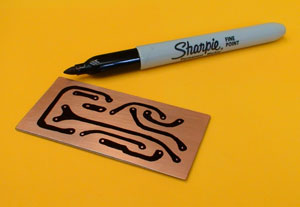
\includegraphics[width=3.15in,height=2.18in]{./media/image6.jpeg}
	\end{Center}
\end{figure}


%%%%%%%%%%%%%%%%%%%% Figure/Image No: 6 Ends here %%%%%%%%%%%%%%%%%%%%

\par

La forma más económica de hacer circuitos impresos es usando la técnica con tinta indeleble. Solo se necesitamos un marcador o plumón de tinta indeleble, como el famoso (Sharpie).\\
Lo primero es dibujar las pistas del circuito sobre la tarjeta, en la cara bañada en cobre. Luego, se sumerge la tarjeta en una solución corrosiva, (cloruro férrico), disuelto en agua caliente. Esta solución corroe la superficie de cobre, dejando sólo el cobre que está cubierto por la tinta del plumón. Para finalizar se perforan con un taladro los orificios donde entrarán las patas de los componentes y listo.\\
Esta técnica por ser netamente manual y con una calidad de impresión regular, se recomienda para hacer circuitos de mediana complejidad, para principiantes o aficionados a la electrónica, que desean realizar pequeños proyectos a muy bajo costo.\par



%%%%%%%%%%%%%%%%%%%% Figure/Image No: 7 starts here %%%%%%%%%%%%%%%%%%%%

\begin{figure}[H]
	\begin{FlushLeft}		
\includegraphics[width=3.15in,height=1.96in]{./media/image7.jpeg}
	\end{FlushLeft}\end{figure}


%%%%%%%%%%%%%%%%%%%% Figure/Image No: 7 Ends here %%%%%%%%%%%%%%%%%%%%

Circuitos impresos elaborados con la técnica de planchado\par

El papel termo transferible es un material utilizado en la elaboración de circuitos impresos de cualquier tipo. Gracias a este papel podemos traspasar a la placa de cobre virgen, el diseño del circuito impreso que hayamos hecho (haya sido hecho a mano o computador), de manera fácil, rápida y económica, para luego introducirla en un recipiente con cloruro ferrico, obteniendo así el circuito impreso deseado. Recomendamos el papel marca (PCBMAKER), aunque también se pueden usar algunos papeles gruesos, usados en dibujo, como el papel Glossy, papel para fotografía o papel Propalcote de unos 120 gramos.\par

Para empezar debemos hacer el circuito del diseño impreso. Este no es otra cosa que el dibujo de las pistas de cobre. El diseño del circuito impreso que hagamos deberá corresponder a las pistas de cobre vistas por $``$transparencia$"$  desde la cara de los componentes (modo espejo).\par



%%%%%%%%%%%%%%%%%%%% Figure/Image No: 8 starts here %%%%%%%%%%%%%%%%%%%%

\begin{figure}[H]
	\begin{Center}
		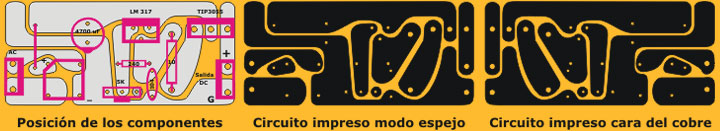
\includegraphics[width=6.95in,height=1.26in]{./media/image8.jpeg}
	\end{Center}
\end{figure}


%%%%%%%%%%%%%%%%%%%% Figure/Image No: 8 Ends here %%%%%%%%%%%%%%%%%%%%

\par

En el momento de hacer el impreso, recuerde que todos nuestros archivos PDF traen el PCB (Print Circuit Board), «Circuito Impreso» al derecho, es decir, vistos por la cara del cobre, pensados para impresión en \href{http://www.construyasuvideorockola.com/fabricacion_impresos_03.php}{Serigrafía} y no tiene necesidad de invertirlo. Si  piensa imprimir el circuito la técnica de Planchado, debe invertirlo (Modo Espejo). Algunos usuarios lo han hecho tal como viene y les queda al revés, por consiguiente pierden el impreso. Para invertir el dibujo del circuito impreso, abra el archivo PDF con Photoshop a una resolución de 300 dpi como mínimo, luego en Menú Imagen (Image) Rotar lienzo (Rotate Canvas), Voltear lienzo horizontal (Flip Canvas Horizontal), se voltea el Impreso horizontalmente a lo largo del eje horizontal.\par



%%%%%%%%%%%%%%%%%%%% Figure/Image No: 9 starts here %%%%%%%%%%%%%%%%%%%%

\begin{figure}[H]
	\begin{Center}
		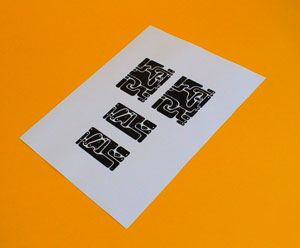
\includegraphics[width=1.68in,height=0.92in]{./media/image9.jpeg}
	\end{Center}
\end{figure}


%%%%%%%%%%%%%%%%%%%% Figure/Image No: 9 Ends here %%%%%%%%%%%%%%%%%%%%

\par

Teniendo hecho el diseño del circuito en el computador, lo imprimimos en alta resolución sobre el papel termo transferible, usando una impresora láser. Se imprime sobre cualquier cara del papel, ya que las dos caras son iguales. Si la imprimimos en un tipo de impresora diferente a láser, el papel termo transferible no servirá (las impresoras láser se reconocen porque utilizan Toner en vez de cartuchos o cintas). Si poseemos el diseño del circuito impreso en una hoja de papel común y corriente o fue hecho a mano, debemos sacar una fotocopia de este, sobre el papel termo transferible. Las fotocopiadoras utilizan el mismo sistema de impresión que las impresoras láser.\par



%%%%%%%%%%%%%%%%%%%% Figure/Image No: 10 starts here %%%%%%%%%%%%%%%%%%%%

\begin{figure}[H]
	\begin{Center}
		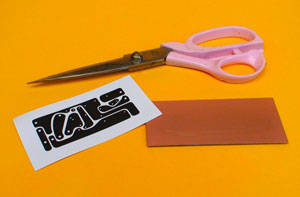
\includegraphics[width=3.15in,height=2.07in]{./media/image10.jpeg}
	\end{Center}
\end{figure}


%%%%%%%%%%%%%%%%%%%% Figure/Image No: 10 Ends here %%%%%%%%%%%%%%%%%%%%

\par

Una vez tengamos el diseño del circuito impreso sobre el papel termo transferible, lo recortamos usando unas tijeras o un bisturí, dejando una margen que nos permita manipularlo. El papel termotransferible restante lo podremos guardar para la elaboración de futuros circuitos impresos.\par



%%%%%%%%%%%%%%%%%%%% Figure/Image No: 11 starts here %%%%%%%%%%%%%%%%%%%%

\begin{figure}[H]
	\begin{Center}
		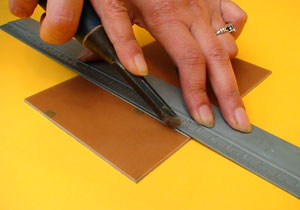
\includegraphics[width=3.15in,height=2.21in]{./media/image11.jpeg}
	\end{Center}
\end{figure}


%%%%%%%%%%%%%%%%%%%% Figure/Image No: 11 Ends here %%%%%%%%%%%%%%%%%%%%

\par

Ahora se debe cortar la placa fenólica a la medida del circuito impreso y posteriormente lavarla por el lado del cobre con jabón desengrasarte de lavaplatos y una esponja de ollas no abrasiva. Seque muy bien la baquelita con un trapo muy limpio o preferiblemente una servilleta desechable. La placa de cobre deberá estar seca, brillante como el oro y limpia de polvo y grasa, además usted No deberá tocar la superficie de cobre con los dedos o cualquier otra cosa.\par



%%%%%%%%%%%%%%%%%%%% Figure/Image No: 12 starts here %%%%%%%%%%%%%%%%%%%%

\begin{figure}[H]
	\begin{Center}
		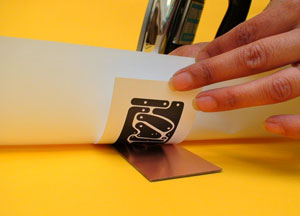
\includegraphics[width=3.15in,height=2.27in]{./media/image12.jpeg}
	\end{Center}
\end{figure}


%%%%%%%%%%%%%%%%%%%% Figure/Image No: 12 Ends here %%%%%%%%%%%%%%%%%%%%

\par

A continuación colocamos la placa sobre una superficie dura, con el lado del cobre mirando hacia arriba. Luego colocamos el papel termo transferible con el diseño del circuito impreso sobre la placa de cobre, de tal manera que el dibujo haga contacto con el cobre. Ahora colocamos una hoja de papel común y corriente, sobre el papel termo transferible.\par

{\fontsize{14pt}{16.8pt}\selectfont Diseño\ de una PCB para el control de un relevador  usando Arduino\par}\par

{\fontsize{14pt}{16.8pt}\selectfont se va a diseñar una PCB de dos capas, para ello se va a trabajar en un circuito que controle un relevador usando la popular plataforma Arduino, el relevador se usa para controlar cargas de corriente alterna o corriente directa.\par}\par

{\fontsize{14pt}{16.8pt}\selectfont Componentes de la PCB y su librería de EAGLE\par}\par

Para iniciar con el diseño de la PCB y más si apenas estamos aprendiendo, conviene identificar las librerías de los componentes, así que es lo que se hará enseguida, por facilidad se va a dividir el circuito en tres partes funcionales, como se observa en la imagen siguiente.\par



%%%%%%%%%%%%%%%%%%%% Figure/Image No: 13 starts here %%%%%%%%%%%%%%%%%%%%

\begin{figure}[H]
	\begin{Center}
		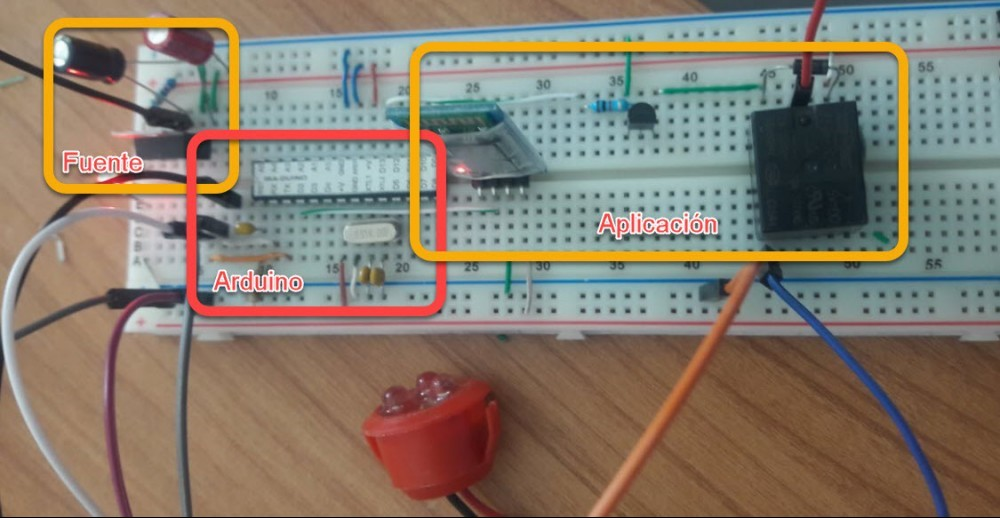
\includegraphics[width=6.61in,height=3.42in]{./media/image13.jpeg}
	\end{Center}
\end{figure}


%%%%%%%%%%%%%%%%%%%% Figure/Image No: 13 Ends here %%%%%%%%%%%%%%%%%%%%

\par

{\fontsize{14pt}{16.8pt}\selectfont \textbf{Fuente de Alimentación}\par}\par

Es la encargada de recibir el voltaje para alimentar el circuito (hasta 12Volts), se forma en esencia por un regulador lineal de voltaje, el popular 7805 para reducir el voltaje a 5 Volts y sus capacitores asociados (2), se agrega un LED con su respectiva resistencia, que enciende cuando se conecta la protoboard a voltaje. La imagen siguiente muestra esta parte.\par



%%%%%%%%%%%%%%%%%%%% Figure/Image No: 14 starts here %%%%%%%%%%%%%%%%%%%%

\begin{figure}[H]
	\begin{Center}
		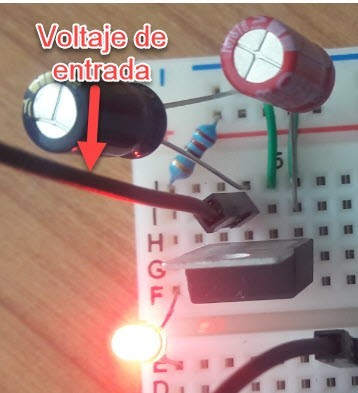
\includegraphics[width=2.54in,height=2.78in]{./media/image14.jpeg}
	\end{Center}
\end{figure}


%%%%%%%%%%%%%%%%%%%% Figure/Image No: 14 Ends here %%%%%%%%%%%%%%%%%%%%

\par

Observe la imagen se remarca un cable que es el de voltaje de entrada de 12 Volts, que viene de la fuente de alimentación, este cable junto con el cable de tierra o GND que no se muestra en la imagen, alimentan al circuito, de alguna forma estos dos cables deben llegar a la PCB para recibirlos usaremos un conector de tornillo (bornera, clema, bloque de terminales o no se como lo conozcas) como los mostrados en la imagen siguiente.\par



%%%%%%%%%%%%%%%%%%%% Figure/Image No: 15 starts here %%%%%%%%%%%%%%%%%%%%

\begin{figure}[H]
	\begin{Center}
		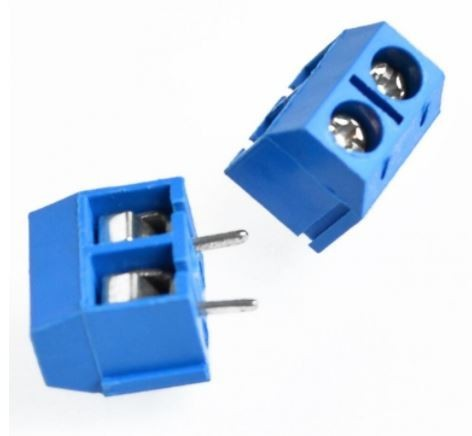
\includegraphics[width=2.7in,height=2.49in]{./media/image15.jpeg}
	\end{Center}
\end{figure}


%%%%%%%%%%%%%%%%%%%% Figure/Image No: 15 Ends here %%%%%%%%%%%%%%%%%%%%

\par

Con lo anterior estaría lista la parte de alimentación de nuestra PCB, lo interesante es ubicar la librería de cada componente que se ve en la protoboard, como se entiende que apenase se está aprendiendo a usar EAGLE, vamos a agregar, a la tabla la librería a usar, recuerde que los componentes todos los que se usan en EAGLE están almacenados en librerías, basta con identificarlos para poder usarlos.\par



%%%%%%%%%%%%%%%%%%%% Table No: 1 starts here %%%%%%%%%%%%%%%%%%%%


\begin{table}[H]
 			\centering
\begin{tabular}{p{1.41in}p{1.92in}p{2.29in}}
\hline
%row no:1
\multicolumn{1}{|p{1.41in}}{\textcolor[HTML]{071136}{Componente}} & 
\multicolumn{1}{|p{1.92in}}{\textcolor[HTML]{071136}{Librería en EAGLE}} & 
\multicolumn{1}{|p{2.29in}|}{\textcolor[HTML]{071136}{Nombre del componente}} \\
\hhline{---}
%row no:2
\multicolumn{1}{|p{1.41in}}{Regulador 7805} & 
\multicolumn{1}{|p{1.92in}}{v-reg.lbr} & 
\multicolumn{1}{|p{2.29in}|}{78XXS} \\
\hhline{---}
%row no:3
\multicolumn{1}{|p{1.41in}}{LED de 3mm} & 
\multicolumn{1}{|p{1.92in}}{Sparkfun-LED.lbr} & 
\multicolumn{1}{|p{2.29in}|}{LED3MM} \\
\hhline{---}
%row no:4
\multicolumn{1}{|p{1.41in}}{Conector de tornillo} & 
\multicolumn{1}{|p{1.92in}}{con-wago-508.lbr} & 
\multicolumn{1}{|p{2.29in}|}{W237-02P} \\
\hhline{---}
%row no:5
\multicolumn{1}{|p{1.41in}}{Resistor de 220 Ohm} & 
\multicolumn{1}{|p{1.92in}}{Sparkfun-Resistor.lbr} & 
\multicolumn{1}{|p{2.29in}|}{1KOHM-HORIZ-1/4W-5$\%$ } \\
\hhline{---}
%row no:6
\multicolumn{1}{|p{1.41in}}{Capacitor de 100 uF} & 
\multicolumn{1}{|p{1.92in}}{SparkFun-Capacitors.lbr} & 
\multicolumn{1}{|p{2.29in}|}{10UF-POLAR-RADIAL-2.5MM} \\
\hhline{---}
%row no:7
\multicolumn{1}{|p{1.41in}}{VCC} & 
\multicolumn{1}{|p{1.92in}}{SparkFun-PowerSymbols.lbr} & 
\multicolumn{1}{|p{2.29in}|}{VCC} \\
\hhline{---}
%row no:8
\multicolumn{1}{|p{1.41in}}{GND} & 
\multicolumn{1}{|p{1.92in}}{SparkFun-PowerSymbols.lbr} & 
\multicolumn{1}{|p{2.29in}|}{GND} \\
\hhline{---}

\end{tabular}
 \end{table}


%%%%%%%%%%%%%%%%%%%% Table No: 1 ends here %%%%%%%%%%%%%%%%%%%%

Se agregan también los símbolos de voltaje y tierra para usarlos en el diagrama esquemático.\par

{\fontsize{14pt}{16.8pt}\selectfont \textbf{Observaciones}\par}\par

\begin{itemize}
	\item La mayoría de las librerías usadas, son diseñadas por la empresa $``$SparkFun$"$  no vienen incluidas en la instalación de EAGLE, pero se pueden descargar desde el siguiente enlace. 
\end{itemize}\par

\href{https://github.com/sparkfun/SparkFun-Eagle-Libraries}{https://github.com/sparkfun/SparkFun-Eagle-Libraries}\par

\begin{itemize}
	\item En la \href{https://pcbcentral.com/pcb-1-adaptador-soic-a-dip-parte-ii-diagrama-esquematico}{lección $\#$ 4 del Nivel I}, al final de la lección, se muestra como almacenar una librería que no viene incluida en EAGLE, por si el lector desea saber la ruta donde se recomienda guardar la librería descargada y como se hace para $``$activarla$"$ . 
\end{itemize}\par

{\fontsize{14pt}{16.8pt}\selectfont \textbf{Componentes Mínimos para el Arduino UNO}\par}\par

Siguiendo con la imagen del diseño, ahora se muestran los componentes mínimos usados para que el ATMEGA funcione en una protoboard.\par



%%%%%%%%%%%%%%%%%%%% Figure/Image No: 16 starts here %%%%%%%%%%%%%%%%%%%%

\begin{figure}[H]
	\begin{Center}
		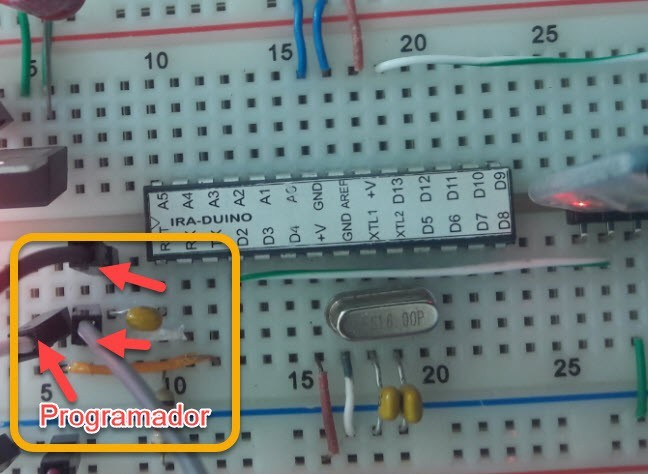
\includegraphics[width=4.02in,height=2.94in]{./media/image16.jpeg}
	\end{Center}
\end{figure}


%%%%%%%%%%%%%%%%%%%% Figure/Image No: 16 Ends here %%%%%%%%%%%%%%%%%%%%

\par

Ahí se muestran todos los componentes necesarios, remarco con flechas como llegan cables ahí son los del programador del Arduino (convertidor USB-Serial) que sirve para transferir el programa al ATMEGA. Para la PCB que estamos diseñando vamos a usar una tira de pines para recibir ahí los cables del programador de Arduino, una tira como esta muy común.\par



%%%%%%%%%%%%%%%%%%%% Figure/Image No: 17 starts here %%%%%%%%%%%%%%%%%%%%

\begin{figure}[H]
	\begin{Center}
		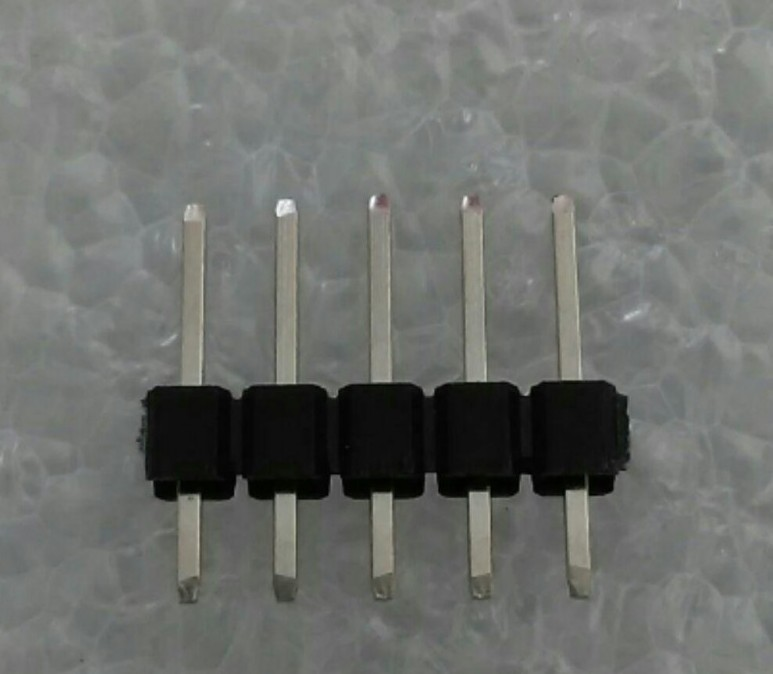
\includegraphics[width=2.84in,height=2.48in]{./media/image17.jpeg}
	\end{Center}
\end{figure}


%%%%%%%%%%%%%%%%%%%% Figure/Image No: 17 Ends here %%%%%%%%%%%%%%%%%%%%

\par

En la siguiente tabla se enumeran cada uno de los componentes de esta parte del diseño, con su respectiva librería.\par



%%%%%%%%%%%%%%%%%%%% Table No: 2 starts here %%%%%%%%%%%%%%%%%%%%


\begin{table}[H]
 			\centering
\begin{tabular}{p{2.18in}p{2.38in}p{2.03in}}
\hline
%row no:1
\multicolumn{1}{|p{2.18in}}{\textcolor[HTML]{071136}{Componente}} & 
\multicolumn{1}{|p{2.38in}}{\textcolor[HTML]{071136}{Librería en EAGLE}} & 
\multicolumn{1}{|p{2.03in}|}{\textcolor[HTML]{071136}{Nombre del componente}} \\
\hhline{---}
%row no:2
\multicolumn{1}{|p{2.18in}}{ATMEGA328P} & 
\multicolumn{1}{|p{2.38in}}{SparkFun-IC-Microcontroller.lbr} & 
\multicolumn{1}{|p{2.03in}|}{ATMEGA328P\_PDIP} \\
\hhline{---}
%row no:3
\multicolumn{1}{|p{2.18in}}{Resistor de 10K} & 
\multicolumn{1}{|p{2.38in}}{Sparkfun-Resistor.lbr} & 
\multicolumn{1}{|p{2.03in}|}{1KOHM-HORIZ-1/4W-5$\%$ } \\
\hhline{---}
%row no:4
\multicolumn{1}{|p{2.18in}}{Capacitor cerámico de 0.1 uF} & 
\multicolumn{1}{|p{2.38in}}{SparkFun-Capacitors.lbr} & 
\multicolumn{1}{|p{2.03in}|}{22PF-PTH-2.54MM} \\
\hhline{---}
%row no:5
\multicolumn{1}{|p{2.18in}}{Cristal de cuarzo (16 MHz)} & 
\multicolumn{1}{|p{2.38in}}{SparkFun-Clocks.lbr} & 
\multicolumn{1}{|p{2.03in}|}{CRYSTAL-16MHZPTH} \\
\hhline{---}
%row no:6
\multicolumn{1}{|p{2.18in}}{Capacitores de 22 pF} & 
\multicolumn{1}{|p{2.38in}}{SparkFun-Capacitors.lbr} & 
\multicolumn{1}{|p{2.03in}|}{22PF-PTH-2.54MM} \\
\hhline{---}
%row no:7
\multicolumn{1}{|p{2.18in}}{Conector para el programador} & 
\multicolumn{1}{|p{2.38in}}{SparkFun-Connectors.lbr} & 
\multicolumn{1}{|p{2.03in}|}{CONN\_05} \\
\hhline{---}

\end{tabular}
 \end{table}


%%%%%%%%%%%%%%%%%%%% Table No: 2 ends here %%%%%%%%%%%%%%%%%%%%

{\fontsize{14pt}{16.8pt}\selectfont \textbf{Componentes para la Aplicación}\par}\par

Finalmente quedan los componentes para la aplicación, que consta del módulo Bluetooth, el relevador y sus componentes asociados, en la imagen siguiente se observan.\par



%%%%%%%%%%%%%%%%%%%% Figure/Image No: 18 starts here %%%%%%%%%%%%%%%%%%%%

\begin{figure}[H]
	\begin{Center}
		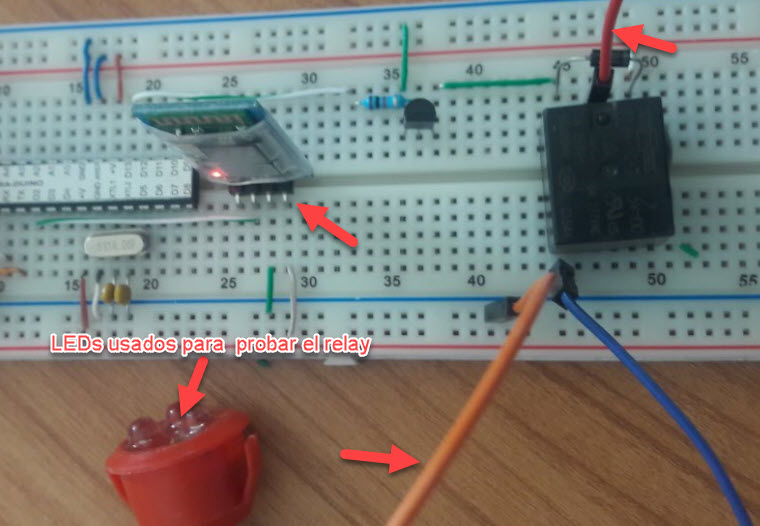
\includegraphics[width=4.48in,height=3.1in]{./media/image18.jpeg}
	\end{Center}
\end{figure}


%%%%%%%%%%%%%%%%%%%% Figure/Image No: 18 Ends here %%%%%%%%%%%%%%%%%%%%

\par

Se remarca con una flecha el Bluetooth, observe que usa pines macho para su conexión, para recibir el módulo en la PCB vamos a usar una tira de pines hembra como la de la siguiente imagen:\par



%%%%%%%%%%%%%%%%%%%% Figure/Image No: 19 starts here %%%%%%%%%%%%%%%%%%%%

\begin{figure}[H]
	\begin{Center}
		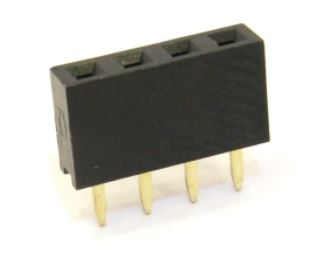
\includegraphics[width=2.29in,height=1.86in]{./media/image19.jpeg}
	\end{Center}
\end{figure}


%%%%%%%%%%%%%%%%%%%% Figure/Image No: 19 Ends here %%%%%%%%%%%%%%%%%%%%

\par

También en la imagen se remarcan dos cables y unos LEDS, se usaron para probar los contactos de salida del relevador,  eso implica pues que tenga que colocar un conector al relevador para llegar con la carga que deseamos controlar, en este caso fueron LEDs, así que se acostumbra usar un conector de tornillo de 3 pines para los contactos del relevador, uno como el mostrado en la imagen siguiente\par



%%%%%%%%%%%%%%%%%%%% Figure/Image No: 20 starts here %%%%%%%%%%%%%%%%%%%%

\begin{figure}[H]
	\begin{Center}
		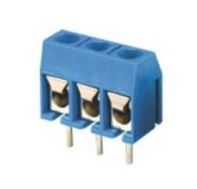
\includegraphics[width=1.81in,height=1.74in]{./media/image20.jpeg}
	\end{Center}
\end{figure}


%%%%%%%%%%%%%%%%%%%% Figure/Image No: 20 Ends here %%%%%%%%%%%%%%%%%%%%

\par

Con esos detalles ya se puede ver en la tabla las librerías necesarias para el diseño de esta parte de la PCB.\par



%%%%%%%%%%%%%%%%%%%% Table No: 3 starts here %%%%%%%%%%%%%%%%%%%%


\begin{table}[H]
 			\centering
\begin{tabular}{p{2.54in}p{1.9in}p{1.97in}}
\hline
%row no:1
\multicolumn{1}{|p{2.54in}}{\textcolor[HTML]{071136}{Componente}} & 
\multicolumn{1}{|p{1.9in}}{\textcolor[HTML]{071136}{Librería en EAGLE}} & 
\multicolumn{1}{|p{1.97in}|}{\textcolor[HTML]{071136}{Nombre del componente}} \\
\hhline{---}
%row no:2
\multicolumn{1}{|p{2.54in}}{Conector para el Módulo Bluetooth} & 
\multicolumn{1}{|p{1.9in}}{SparkFun-Connectors.lbr} & 
\multicolumn{1}{|p{1.97in}|}{CONN\_05} \\
\hhline{---}
%row no:3
\multicolumn{1}{|p{2.54in}}{Relevador} & 
\multicolumn{1}{|p{1.9in}}{Relay.lbr} & 
\multicolumn{1}{|p{1.97in}|}{G5L} \\
\hhline{---}
%row no:4
\multicolumn{1}{|p{2.54in}}{Transistor 2N2222} & 
\multicolumn{1}{|p{1.9in}}{SparkFun-DiscreteSemi.lbr} & 
\multicolumn{1}{|p{1.97in}|}{TRANS\_NPN-2N3904} \\
\hhline{---}
%row no:5
\multicolumn{1}{|p{2.54in}}{Diodo 1N4001} & 
\multicolumn{1}{|p{1.9in}}{SparkFun-DiscreteSemi.lbr} & 
\multicolumn{1}{|p{1.97in}|}{DIODE-1N4148} \\
\hhline{---}
%row no:6
\multicolumn{1}{|p{2.54in}}{Resistor de 1K} & 
\multicolumn{1}{|p{1.9in}}{Sparkfun-Resistor.lbr} & 
\multicolumn{1}{|p{1.97in}|}{1KOHM-HORIZ-1/4W-5$\%$ } \\
\hhline{---}
%row no:7
\multicolumn{1}{|p{2.54in}}{Bloque de terminales (3 posiciones)} & 
\multicolumn{1}{|p{1.9in}}{con-wago-508.lbr} & 
\multicolumn{1}{|p{1.97in}|}{W237-3E} \\
\hhline{---}

\end{tabular}
 \end{table}


%%%%%%%%%%%%%%%%%%%% Table No: 3 ends here %%%%%%%%%%%%%%%%%%%%


\vspace{\baselineskip}
Con esta lección se deja todo listo para iniciar con el diseño del diagrama esquemático en EAGLE.\par

{\fontsize{15pt}{18.0pt}\selectfont \textbf{\textcolor[HTML]{000080}{Bibliografía: }}\par}\par

\href{https://pcbcentral.com/pcb-2-diseo-de-una-pcb-para-el-control-de-un-relevador-por-bluetooth-usando-arduino}{{\fontsize{14pt}{16.8pt}\selectfont https://pcbcentral.com/pcb-2-diseo-de-una-pcb-para-el-control-de-un-relevador-por-bluetooth-usando-arduino}\par}\par

\href{https://www.inventable.eu/controlar-rele-con-transistor/}{{\fontsize{14pt}{16.8pt}\selectfont https://www.inventable.eu › controlar-rele-con-transistor}\par}\par


\printbibliography
\end{document}